\subsection{jPerf}

\subsection{BR1-S2 nach AS2}
\begin{figure}[h]
	\centering
	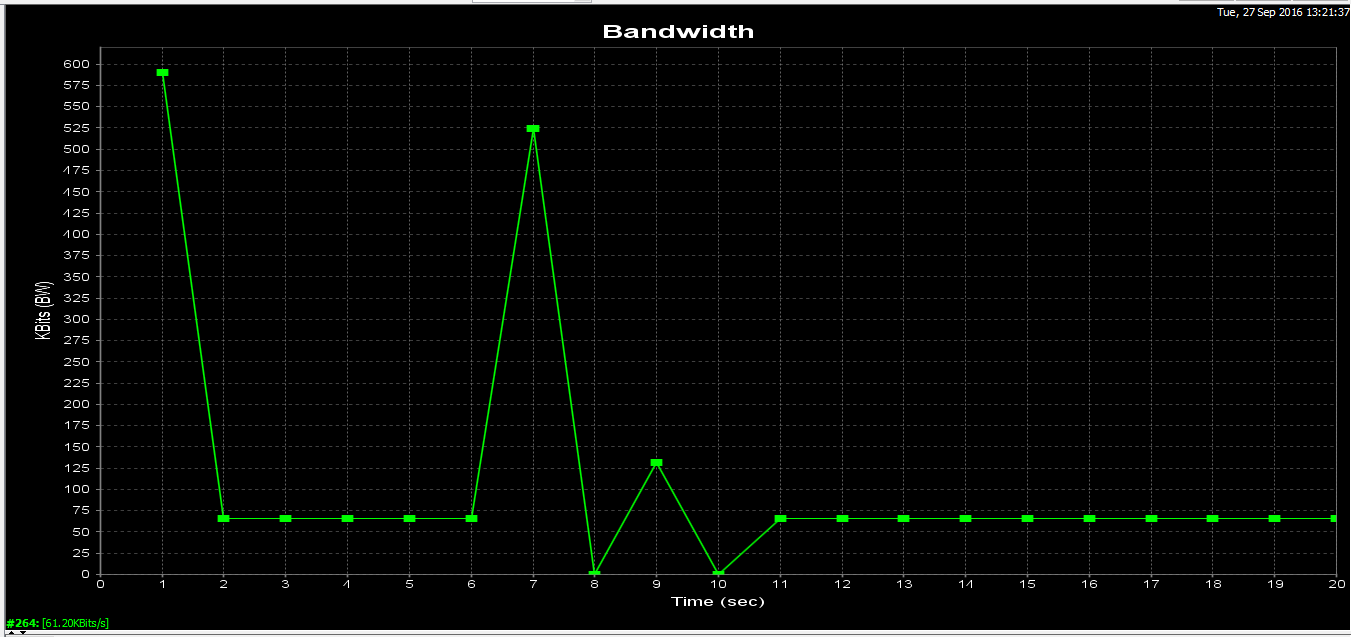
\includegraphics[width=0.7\linewidth]{appendix/measurements/jperf/br1-s2-to-as2}
	\caption{jPerf Graph von BR1-S2 nach AS2}
	\label{fig:as2-to-as6}
\end{figure}

\subsection{AS2 nach AS6}
\begin{figure}[h]
\centering
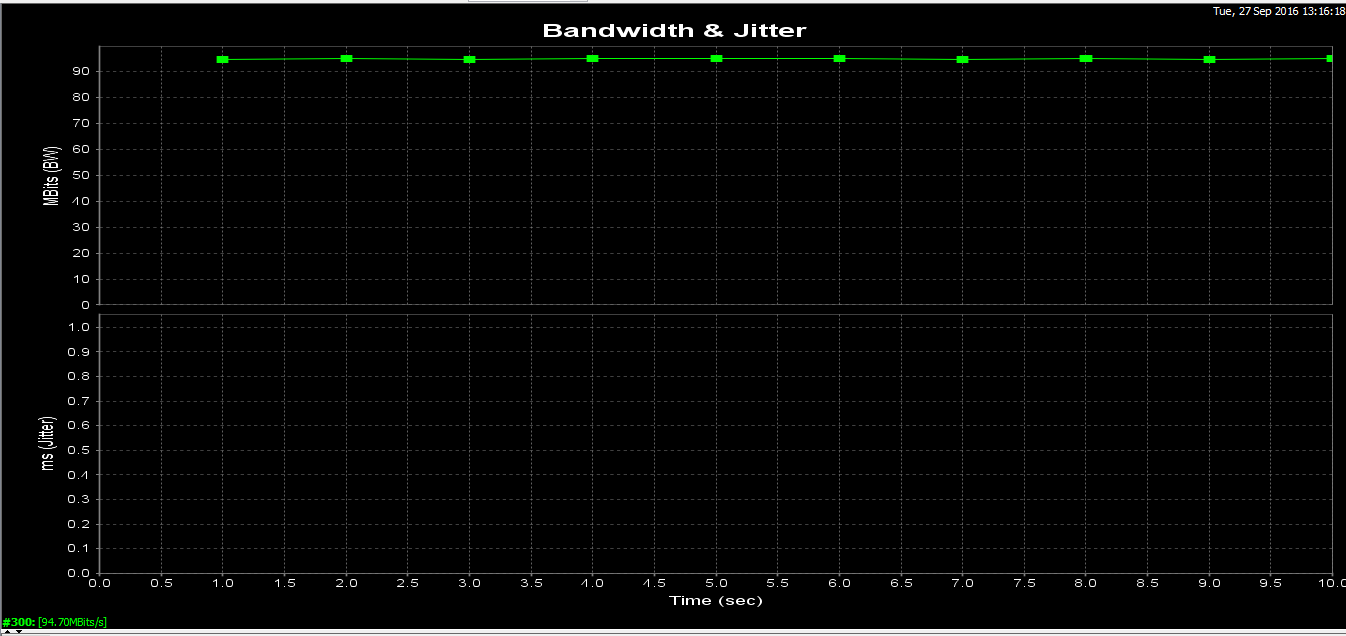
\includegraphics[width=0.7\linewidth]{appendix/measurements/jperf/as2-to-as6}
\caption{jPerf Graph von AS2 nach AS6}
\label{fig:as2-to-as6}
\end{figure}



\subsection{Traceroutes}
\subsubsection{HQ-AS2 nach BR1-S1 via FRR}
\lstinputlisting{appendix/measurements/traceroute/hq-as2-to-br1-s1-via-frr.txt}

\subsubsection{HQ-DS3 nach BR1-S1 via FRR}
\lstinputlisting{appendix/measurements/traceroute/hq-ds3-to-br1-s1-via-frr.txt}

\subsubsection{HQ-AS2 nach BR2-S1 via IER1}
\lstinputlisting{appendix/measurements/traceroute/hq-as2-to-br2-s1-via-ier1.txt}

\subsubsection{IER1 nach BR1-SR1}
\lstinputlisting{appendix/measurements/traceroute/ier1-to-br1-sr1.txt}

\subsubsection{AS6 nach AS2}
\lstinputlisting{appendix/measurements/traceroute/as6-to-as2.txt}

\subsubsection{172.16.100.2}
\lstinputlisting{appendix/measurements/traceroute/172-16-100-2.txt}

\subsubsection{172.16.102.2}
\lstinputlisting{appendix/measurements/traceroute/172-16-102-2.txt}


\subsection{Pings}
\subsubsection{FRR nach BR1-SR1}
\lstinputlisting{appendix/measurements/ping/frr-to-br1-sr1.txt}


\subsubsection{FRR nach BR2-SR1}
\lstinputlisting{appendix/measurements/ping/frr-to-br2-sr1.txt}



